\section{Progetto CTMC}

La prima parte del progetto che ho realizzato è un simulatore per modelli
CTMC utilizzando il linguaggio Maude e le sue funzionalità di meta-livello.

\subsection{Requisiti}
\label{sec:requisiti}

Si vuole realizzare un simulatore per catene di Markov tempo continue in grado
di:
\begin{itemize}
  \item Gestire stati arbitrari.
  \item Gestire azioni di transizione da uno stato all'altro caratterizzate da
  un certo rate, permettendo di specificare condizioni e rate dinamici.
  \item Gestire delle overview, ovvero risultati parziali dell'esecuzione.
\end{itemize}

\subsection{Realizzazione}

Una transizione è descrivibile come $State \Longrightarrow [Rate] State$ $if$
 $Condition$, ovvero come stati che possono essere trasformati in altri stati
secondo un certo rate e se è avverata una data condizione. Questa definizione è
naturalmente riconducibile alle \emph{rewriting rule} di Maude; dunque, definita
una sintassi per i membri delle rule, si può sfruttare il meccanismo di rewrite
nativo.

L'ultimo punto dei requisiti riguarda la gestione delle overview. Definisco una
Overview come una informazione che l'utente riceve ogni $M$ passi di
simulazione, contenente informazioni relative alla dinamica del sistema.

\subsection{Organizzazione}

Il sistema è suddiviso in due moduli. \emph{CTMC} contiene per la sintassi
di CTMC, che i moduli utente devono importare, mentre \emph{CTMC-ENGINE}
contiene le operazioni necessarie per la simulazione.

\subsubsection{Modulo CTMC}

All'interno del modulo \emph{CTMC} ho definito i Sort e i costruttori del
modello CTMC. Una catena di Markov è una coppia $\langle A , \rightarrow A
\rangle$, dove $A$ è un insieme di stati e $\rightarrow \subseteq A \times
\mathbb{R}_{0}^{+} \times A$ è una transizione fra due stati che avviene con un
certo rate. Come detto precedentemente, è possibile sfruttare il meta-livello di
Maude per gestire le transizioni come \emph{rule} e definire unicamente la sintassi.

Per avere una definizione più generica possibile di stato del sistema, definisco
uno \emph{State} come un elemento polimorfico:
\begin{Verbatim}[fontsize=\small]
sort State  .
op <_> : Universal -> State [ ctor poly (1) ] .
\end{Verbatim}

Per modellare i rate, ho definito un sort che comprenda rate e stato finale e
che possa essere riscritto dallo stato inziale: \emph{Config} subsort di
\emph{State}. In questo modo \emph{State} può essere riscritto come un
\emph{Config}.
\begin{Verbatim}[fontsize=\small]
sort Config Rate Var .
subsort Float < Rate .
subsort Config < State .
op [_]_ : Rate State -> Config [ ctor prec 80 ] .
\end{Verbatim}
Per semplificare ed ottimizzare le operazioni di simulazione, impongo che il
modulo utente debba definire le regole di rewrite del modello con la
label \emph{model}. Ad esempio:
\begin{Verbatim}[fontsize=\small]
*** Esempio di modello CTMC in cui lo stato è un multi-set
*** di numeri naturali. Le regole che formano il modello devono
*** avere la label model.

sort NatMSet .
subsort Nat < NatMSet .
op nil : -> NatMSet .
op __ : NatMSet NatMSet -> NatMSet [ ctor comm assoc id: nil ] .

crl [model] : < 12 N:Nat 123 > =>
                   [0.2 * float(N:Nat)] < 1312 > if N:Nat > 14 .
crl [model] : < N:Nat > =>
                   [0.8 * float(N:Nat)] < 12 15 123 > if N:Nat > 1300 .
rl [model] : < N:Nat NL:NatList > =>
                   [12.0] < (N:Nat + 1) NL:NatList > .
\end{Verbatim} 

Nel modulo \emph{CTMC} ho anche definito la sintassi per l'overview,
implementato come contenitore di una lista di \emph{Entry}, coppie
$(Tempo, Stato)$:
\begin{Verbatim}[fontsize=\small]
sort Overview Entry EntryList .
subsort Entry < EntryList .

op _:_ : Float State -> Entry [ ctor prec 80 ] .
op empty : -> EntryList [ ctor ] .
op _ - _ : EntryList EntryList -> EntryList [ ctor assoc id: empty prec 90 ] .
op [_] : EntryList -> Overview [ ctor ] .
\end{Verbatim}

Per i motivi che spiegherò in seguito, il modulo utente per la gestione
dell'overview, deve implementare un sistema di rule per riscrivere l'Overview,
tenendo conto che sarà effettuata un'unica rewrite . Per iterare l'overview si
possono comunque usare sistemi di equazioni, poiché il risultato è sempre
ridotto.

\subsubsection{Modulo CTMC-ENGINE}
\label{sec:CTMC-ENGINE}

Il modulo engine è il simulatore dei modelli CTMC. Ho realizzato questo engine
in modo che potesse simulare dinamicamente un modello, ricevendo il nome del
modulo che lo implementa e la meta-rappresentazione dello stato iniziale. In
questo modo non ha bisogno di conoscere operazioni ed sort del modulo
utente.

Utilizzando l'operazione \emph{upModule}, descritta nella sezione
\ref{sec:upMod}, il simulatore è in grado di ottenere il meta-modulo e
cominciare la simulazione eseguendo ricorsivamente una sequenza di passi:

\begin{enumerate}
  \item Trovare tutte le azioni concorrenti che possono attivarsi dallo stato
  corrente.
  \item Scegliere una azione $a_i$ con probabilità $\frac{r_i}{R}$, dove $R =
  \sum_i{r_i}$
  \item Applicare l'azione, determinando il nuovo stato del sistema.
  \item Incrementare il tempo di $\Delta{}t = \frac{1}{R}\log{\frac{1}{\tau}}$,
  dove $\tau = random(0, 1)$ .
  \item Appendere il nuovo risultato all'overview e controllare se occorre
  comunicarlo all'utente.
\end{enumerate}

Tutti i passi sono realizzati utilizzando il meta-livello di Maude e i dati di
stato ed overview sono trattati in forma non-canonica, quindi quando scrivo
\emph{stato} ed \emph{overview} in realtà intendo le loro meta-rappresentazioni.

Il passo 1 è facilmente risolto imponendo al modulo utente di etichettare tutte
le rule con la label \emph{model}. Grazie a questo vincolo è possibile
utilizzare ricorsivamente la \emph{metaXapply}; incrementando di volta in volta
l'ultimo parametro (vedi sezione \ref{sec:mapply}), si possono iterare tutte le
soluzioni possibili scartando quelle già ottenute. Le soluzioni sono tutte le
riscritture valide a partire dallo stato corrette. Per avere la sicurezza di una
riscrittura completa, impongo che il Context, ovvero la sequenza di termini non
riscritti dalla rule, sia vuoto.

Come strutture di supporto, dichiaro tre sort:
\begin{Verbatim}[fontsize=\small]
*** Action -> possibile rewrite, memorizza rate e meta-stato finale
*** ActionList -> Lista di azioni
*** TotalActions -> composto dalla lista delle azioni e dalla
***                                              somma dei loro rate
sort Action ActionList TotalActions .
subsort Action < ActionList .

op ac : Float Term -> Action .
op nil : -> ActionList .
op _ ; _ : ActionList ActionList -> ActionList [ ctor assoc id: nil prec 110 ]  .
*** Definisce un TotalAction (somma dei rate e action list)
op acts : Float ActionList -> TotalActions [ ctor ] .
*** Operazioni di utilità per concatenare e aggiungere Azioni
*** a TotalAction
op _+_ : TotalActions TotalActions -> TotalActions .
op _#_ : TotalActions Action -> TotalActions [ prec 90 ] .
\end{Verbatim}
\emph{Action} è una struttura di supporto che rappresenta un \emph{Config},
ovvero un $[Rate] State$, definito nel modulo CTMC. \emph{Action} memorizza il
rate in forma canonica e il meta-stato come \emph{Term}.
\emph{ActionList} è una lista di \emph{Action} e \emph{TotalAction} è un
contenitore di una \emph{ActionList} e della somma dei rate delle singole
\emph{Action}.

Per eseguire ricorsivamente la \emph{metaXapply} e riempire un TotalAction,
ho definito l'operazione \emph{applyAll}, di cui riporto anche
l'implementazione, poiché è significativa nell'uso del meta-livello.

\begin{Verbatim}[fontsize=\small]
*** Costruisce la TotalActions contenente tutte le azioni
*** possibili a partire dal dato stato iniziale. Funzione tail.
op applyAll : Module Term TotalActions Nat -> TotalActions .

*** meta-applico ricorsivamente la rule "model" incrementando
*** il numero di soluzioni da scartare: così ottenengo tutte
*** le soluzioni possibili. 
*** Il risultato della metaXApply è composto da 4 termini.
*** Due non sono utilizzati, gli altri due sono:
***	   * Term -> meta-Config risultato dall'applicazione della rule
***	   * Context -> lista dei termini non riscritti.
***                  Deve essere vuota ( '[]' )
***
ceq applyAll(Mod, S, acts(SumR, AL), ResIdx) = 
        *** Ricorsione appendendo le ActionList
        applyAll(Mod, S, acts(SumR, AL) # ac(R2, S2), ResIdx + 1)
        *** Eseguo la metaXapply
    if  result? := metaXapply(Mod, S, 'model , none, 0, unbounded, ResIdx) /\
        *** Controllo che sia andato tutto bene e che il context sia vuoto
        result? :: Result4Tuple /\ getContext(result?) == [] /\
        *** '`[_`]_[RT, S2] è il meta-config riscritto ([RT] S2)
        '`[_`]_[RT, S2] := getTerm(result?) /\
        R2 := downTerm(RT, 0.0) .
\end{Verbatim}

Ottenute tutte le possibili azioni, bisogna sceglierne una casualmente, sulla
base del rate (passo 2). Questo può essere implementato generando un numero
casuale fra 0 e la somma dei rate e scegliendo una \emph{Action} trattando i
corrispettivi rate come se fossero delle probabilità.
\begin{Verbatim}[fontsize=\small]
*** Dato l'indice della sequenza di numeri random, ritorna un
*** valore casuale compreso fra 0 e 1 estremi inclusi.
op rand : Nat -> Float .

*** Sceglie un'azione sulla base del rate
op pickOne : ActionList Float Float -> Action .
\end{Verbatim}

Ottenuta la action, l'estrazione dello stato finale è banale (passo 3):
\begin{Verbatim}[fontsize=\small]
*** Ricava dall'azione il meta-stato finale
op mineAction : Action -> Term .
eq mineAction(ac(R, S)) = S .
\end{Verbatim}

Terminato il passo di simulazione, occorre aggiornare l'overview ed
eventualmente comunicarlo all'utente (passo 4). Ovviamente anche l'overview deve
essere trattato al meta-livello, quindi l'append progressiva di \emph{Entry}
alla \emph{EntryList} avviene così:
\begin{Verbatim}[fontsize=\small]
*** ELTmp è il nuovo meta-EntryList 
*** ELI è il meta-EntryList (Term) dello stato precedente 
*** TimeF è il nuovo tempo
*** StateF è il nuovo meta-stato

ELTmp := '_-_[ELI , '_:_[upTerm(TimeF), StateF]]
\end{Verbatim}

Per quando riguarda la comunicazione dell'Overview, ho implementato
una rewrite con profondità 1 dell'overview sul modulo utente. L'utente può
sfruttare quell'unica rewrite (si ricorda che la rewrite automaticamente riduce
tutti i termini), per stampare i risultati a video. L'overview riscritta diventa
l'overview iniziale per gli step successivi. Questa scelta motiva la struttura
dell'overview come contenitore di entry-list e non solo come entry-list, poiché
una rewrite può avvenire anche su sottosequenze di una lista.

Anche in questo caso è necessario l'utilizzo del meta-livello per effettuare una
\emph{metaRewrite} dinamicamente sul modulo utente.
\begin{Verbatim}[fontsize=\small]
***
*** Controlla se occorre riscrivere l'overview nel modulo utente.
*** Ritorna la meta-EntryList a cui appendere i risultati successivi. 
***   Module -> meta-modulo utente .
***   Term -> meta-EntryList .
***   Nat -> step di simulazione corrente.
***   Nat -> Overview size
op checkOverview : Module Term Nat Nat -> Term .
\end{Verbatim}

\subsection{Simulazione}

I passi di simulazione elencati nella sezione precedente (\ref{sec:CTMC-ENGINE})
sono svolti ricorsivamente da un insieme di operazioni \emph{simulate} che ho
implementato come un sistema di equazioni. La simulazione termina o al
compimento dei passi richiesti o al raggiungimento di un deadlock, ritornando un
SimulationResult, che contiene il tempo, lo stato corrente ed un booleano che
vale true se è stato raggiunto un deadlock.
\begin{Verbatim}[fontsize=\small]
*** SimulationResult -> composto da tempo + meta-stato corrente + deadlock?
sort SimulationResult .
op sim : Float Term Bool -> SimulationResult [ ctor ] .
\end{Verbatim}

Per avviare la simulazione si deve ridurre una operazione di entry point
\emph{simulate} a 5 argomenti, la quale richiama la \emph{simulate} a 8
argomenti che esegue la simulazione ricorsiva.
\begin{Verbatim}[fontsize=\small]
***
*** Wrapper per la simulazione
***     Qid -> Nome del modulo utente.
***     Term -> meta-stato iniziale.
***     Nat -> Numero di passi di simulazione desiderati.
***     Nat -> Ogni quanti passi ricevere l'overview
***            (0 se non si vuole gestire l'Overview).
***     Nat -> Indice per la generazione dei numeri random
***                                        da cui iniziare.
op simulate : Qid Term Nat Nat Nat -> SimulationResult .
	
***
*** Operazione di simulazione da usare ricorsivamente.
***     Module -> meta-modulo utente.
***     SimulationResult -> risultato parziale.
*** 	Nat -> Numero di step totali.
***		Nat -> Numero di step effettuati.
***     Bool -> true se l'utente vuole ricevere l'overview.
***     Nat -> Dimensione target dell'overview.
***     EntryList -> contenuto dell'Overview
***     Nat -> Indice per la generazione dei numeri random .
op simulate : Module SimulationResult Nat Nat
          Bool Nat Nat EntryList Nat -> SimulationResult .
\end{Verbatim}

Riporto l'implementazione dell'operazione di simulazione ricorsiva, mostrando i
passi descritti nella sezione \ref{sec:CTMC-ENGINE}.

\begin{Verbatim}[fontsize=\small]

var Mod : Module .
var A : Action .
var StateI StateF : Term .
var AL : ActionList .
var RandIdx Step OvSize MaxStep : Nat .
var SumR TimeI TimeF Tau1 Tau2 : Float .
var ELI ELF : Term .
var memOv : Bool .

ceq simulate(Mod, sim(TimeI, StateI, false), MaxStep, Step, memOv,
                                          OvSize, ELI, RandIdx) =
    simulate(Mod, sim(TimeF, StateF, false), MaxStep, Step + 1, memOv,
                                        OvSize, ELF, RandIdx + 2)
        *** Passo 1
    if  acts(SumR, AL) := applyAll(Mod, StateI) /\ SumR > 0.0 /\
        *** Passo 2
        Tau1 := rand(RandIdx) /\ Tau2 := rand(RandIdx + 1) /\
        A := pickOne(AL, SumR * Tau1, 0.0) /\
        *** Passo 3
        StateF := mineAction(A) /\
        TimeF := TimeI + log(1.0 / Tau2) / SumR /\
        *** Passo 4
        ELF := ( if memOv
                 then checkOverview(Mod,
                    '_-_[ELI , '_:_[upTerm(TimeF), StateF]], Step + 1, OvSize)
                 else
                    'empty.EntryList
               fi) .
\end{Verbatim}

\emph{Nota:} ho progettato il simulatore per essere il più generale possibile,
perciò delego all'utente finale il compito di scrivere dei wrapper per non dover
avviare la simulazione specificando i meta-stati anziché gli stati.

\subsection{Modelli di esempio}
\label{sec:esempio}

Di seguito riporto tre modelli CTMC implementati utilizzando il framework. In
tutti i modelli ho condiviso un Sort che definisce liste di oggetti \emph{Var},
che rappresentano variabili identificate da un nome e a cui è associato un
valore:
\begin{Verbatim}[fontsize=\small]
***
*** Modulo di utilità, definisce liste di variabili da poter
*** utilizzare come state.
***
fmod CTMC-EXTRA is
	
	pr CTMC .

	sort Var VarList .
	subsort Var < VarList .
	
	op null : -> VarList .
	op __ : VarList VarList -> VarList [ ctor assoc comm id: null ] .
	op v : String  Universal -> Var [ ctor poly (2) ] .

endfm
\end{Verbatim}

\subsubsection{Modello Readers-Writers}
\label{sec:rw}
Il modello readers and writers rappresenta un sistema concorrente in cui $N$
processi accedono ad una risorsa condivisa in lettura o scrittura. La lettura è
shared, la scrittura exclusive.  In figura \ref{petri2} è  mostrata la rete di
petri che lo implementa.

\begin{figure}[!hb]
	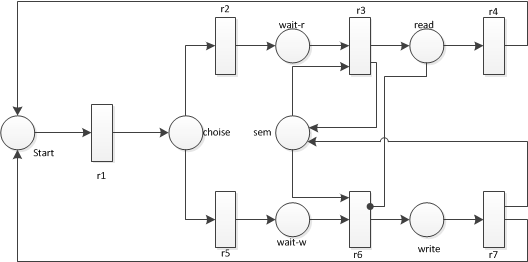
\includegraphics[width=10cm]{../resources/images/petri2.png}
	\label{petri2}
	\caption{Rete di petri simulata da CTMC-READER\_WRITER}
\end{figure}

Il modello si può esprimere in modo stocastico, facendo dipendere dal numero di
token i rate da un place all'altro. Implementativamente, per rapprentare gli
stati si utilizza un set di variabili, una per place, che hanno come valore il
numero di token.
\begin{Verbatim}[fontsize=\small]
var VL : VarList .
var N, M : Nat .

*** Start
crl [model] : < v("start" , N) v("choose" , M) VL > =>
             [10.0 * float(N)]
               < v("start" , N + -1) v("choose" , M + 1) VL >
             if N > 0 .
*** Read
crl [model] : < v("choose" , N) v("waitr" , M) VL > =>
             [5.0 * float(N)]
               < v("choose" , N + -1) v("waitr" , M + 1) VL >
             if N > 0 .
crl [model] : < v("waitr" , N) v("read" , M) v("sem" , 1) VL > =>
             [20.0 * float(N)]
               < v("waitr" , N + -1) v("read" , M + 1) v("sem" , 1) VL >
             if N > 0 .
crl [model] : < v("read" , N) v("start" , M) VL > =>
             [50.0 * float(N)]
               < v("read" , N + -1) v("start" , M + 1) VL >
             if N > 0 .
*** Write
crl [model] : < v("choose" , N) v("waitw" , M) VL > =>
             [5.0 * float(N)]
               < v("choose" , N + -1) v("waitw" , M + 1) VL >
             if N > 0 .
crl [model] : < v("waitw" , N) v("write" , M) v("sem" , 1)
                                            v("read" , 0) VL > =>
             [40.0 * float(N)]
               < v("waitw" , N + -1) v("write" , M + 1)
                                               v("sem" , 0) v("read" ,0) VL >
             
             if N > 0 .
crl [model] : < v("write" , N) v("start" , M) v("sem" , 0) VL > =>
             [50.0 * float(N)]
               < v("write" , N + -1) v("start" , M + 1) v("sem" , 1) VL >
             if N > 0 .

\end{Verbatim}

\subsubsection{Modello M/M/C/K per la simulazione delle code}
\label{sec:mmck}

M/M/C/K è un modello utilizzato nella teoria delle code per analizzare e
simulare il comportamento di un sistema di $C$ server che elaborano un task
alla volta. I task nascono con un certo rate $\tau$ e sono memorizzati in un
buffer di dimensione $K$. Se il buffer è pieno sono perduti. I task muoiono
(sono svolti dai server) con un rate che vale $\mu * N$, dove N è il numero dei
task, se $N \leq C$, altrimenti il rate vale $\mu * C$.

Gli stati del modello sono enumerabili da un numero naturale, tuttavia nel
modello sono inclusi anche altri elementi di configurazione ed utilità come la
dimensione del buffer, il numero di server e il numero di task perduti.

\begin{Verbatim}[fontsize=\small]
var N K L C : Nat .
var VL : VarList .

*** Accodamento nel Buffer
crl [model] : < v("buffersize" , K) v("buffer", N) VL > =>
              [ 0.535 ] < v("buffersize" , K) v("buffer", N + 1) VL >
              if N < K .
*** Buffer pieno
crl [model] : < v("buffersize" , K) v("buffer", N) v("losts", L) VL > =>
              [ 0.535 ] < v("buffersize" , K) v("buffer", N)
                                               v("losts", L + 1) VL >
              if N >= K .
*** Svolgimento di task (caso N < C)
crl [model] : < v("nserver" , C) v("buffer", N) VL > =>
              [0.120 * float(N)] < v("buffer", N + -1) v("nserver" , C) VL >
              if N > 0 /\ N < C .
*** Svolgimento di task (caso N >= C)
crl [model] : < v("nserver" , C) v("buffer", N) VL > =>
              [0.120 * float(C)] < v("buffer", N + -1) v("nserver" , C) VL >
              if N > 0 /\ N >= C .

\end{Verbatim}

\subsection{Modello di test della Bromosulftaleina}
\label{sec:bsf}

\begin{figure}[!ht]
	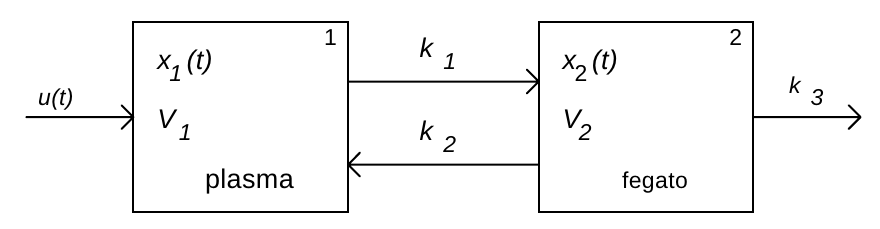
\includegraphics[width=10cm]{../resources/images/BSF.png}
	\label{bsf}
	\caption{Modello BSF (\cite{gnudi})}
\end{figure}

Il test BSF \cite{gnudi} è semplificabile considerandolo un sistema a due compartimenti
(uno per il fegato, l'altro per il plasma), con un certo rate di trasferimento. Si
suppone un inserimento del colorante nel plasma istantaneo e si può
semplificarlo imponendo la condizione inziale del plasma pari alla quantità di
colorante iniettato. Il colorante, quando entra nel fegato, scompare con un
certo rate e è riassorbito nel plasma con un altro rate. Per completezza si
considera anche il volume dei due compartimenti (vedi figura \ref{bsf}).

Il modello è semplificato al caso di trasferimenti di colorante discreti.

\begin{Verbatim}[fontsize=\small]
var N K L : Nat .
var VP VF : Nat .
var VL : VarList .
	
	
*** Passaggio colorante dal compartimento plasma a fegato
crl [model] : < v("volplasma", VP) v("volfegato", VF)
                       v("plasma", N) v("fegato", L) > =>
              [ 0.454 * float(N) / float(VP) ]
              < v("volplasma", VP) v("volfegato", VF)
                v("plasma", N + -1)  v("fegato", L + 1) >
              if N > 0 /\ L < VF .

*** Passaggio colorante dal compartimento fegato a plasma            
crl [model] : < v("volfegato", VF) v("volplasma", VP)
                       v("plasma", N) v("fegato", L) > =>
             [ 0.698 * float(L) / float(VF) ]
             < v("volfegato", VF) v("volplasma", VP)
               v("plasma", N + 1) v("fegato", L + -1) >
             if L > 0 /\ N < VP .
		
*** Scomparsa del colorante dal compartimento fegato
crl [model] : < v("volfegato", VF) v("fegato", L) VL > =>
             [ 0.432 * float(L) / float(VF) ]
             < v("volfegato", VF) v("fegato", L + -1) VL >
             if L > 0 .
	
\end{Verbatim}